\documentclass[a4paper,12pt]{report}
\usepackage[spanish,activeacute]{babel}
\usepackage[utf8]{inputenc}
\usepackage{graphicx}
\usepackage{eurosym}
\usepackage{url}
\renewcommand\thesection{\arabic{section}}


\usepackage[T1]{fontenc}
\usepackage{times}
\usepackage[toc,page]{appendix}

\usepackage{verbatim} % comentarios

\usepackage{color}
\definecolor{gray97}{gray}{.97}
\definecolor{gray75}{gray}{.75}
\definecolor{gray45}{gray}{.45}

\usepackage{listings}
\lstset{ frame=Ltb,
	framerule=0pt,
	aboveskip=0.5cm,
	framextopmargin=3pt,
	framexbottommargin=3pt,
	framexleftmargin=0.4cm,
	framesep=0pt,
	rulesep=.4pt,
	backgroundcolor=\color{gray97},
	rulesepcolor=\color{black},
	%
	stringstyle=\ttfamily,
	showstringspaces = false,
	basicstyle=\small\ttfamily,
	commentstyle=\color{gray45},
	keywordstyle=\bfseries,
	%
	numbers=left,
	numbersep=15pt,
	numberstyle=\tiny,
	numberfirstline = false,
	breaklines=true,
}

% minimizar fragmentado de listados
\lstnewenvironment{listing}[1][]
{\lstset{#1}\pagebreak[0]}{\pagebreak[0]}

\lstdefinestyle{consola}
{basicstyle=\scriptsize\bf\ttfamily,
	backgroundcolor=\color{gray75},
}

\lstdefinestyle{C}
{language=C,
}



\begin{document}
	
	\pagestyle{empty}
	\begin{titlepage}
		\begin{center}
			
\includegraphics[scale=0.15]{images/fic01.png} \\ 
			\vspace{2cm} 
\includegraphics[scale=.4]{images/udc.pdf} \\
			
			
			\vspace{2.5cm}
			
			\textbf{\Large Diseño Software en un Quake III Arena}\\
			\vspace{0.5cm}
			\large{Máster Universitario en Ingeniería Informática}\\
		\end{center}
		
		\vspace{7.2cm}
		\begin{flushright}
			\noindent Elena M. Delamano Freije
			
			\noindent Martín Álvarez Castillo
			
		\end{flushright}
	\end{titlepage}
	\clearpage
	
	
	\tableofcontents
	\clearpage
	
	
	\section{Introducción}
	Quake III Arena, a partir de ahora referido como \textbf{Q3}, es un videojuego de disparos en primera persona (\textit{FPS}) que fue lanzado en el año 1999 por \textit{id Software}. Este anticipado lanzamiento, al igual que el resto de juegos de \textit{id}, revolucionó el género de los FPS, tanto a nivel de diseño \,---\,el cual no se comentará en este documento, excepto donde sea relevante\,---\,, como a nivel de tecnologías e implementación de motor gráfico de tiempo real en el ámbito de los videojuegos. \cite{quake3}\\
	
	El nuevo motor desarrollado para crear Q3 fue bautizado como \textit{id tech 3}. Cuando existan referencias a Q3 en esta memoria, realmente se estará haciendo referencia a la versión de \textit{id tech 3} empleada para el desarrollo de Q3. Para desarrollos comerciales, \textit{id Software} ofreció una licencia de su nuevo motor a empresas de terceros. Una de las múltiples empresas que licenció \textit{id tech 3} fue Activision, para el desarrollo de la primera edición de \textit{Call of Duty}. La licencia del motor permitía la modificación del mismo y, a día de hoy, la familia de juegos de la franquicia de \textit{Call of Duty} todos usan una versión modificada cuya raíz es \textit{id tech 3}. \cite{idtech3}\\
	
	Asimismo, siguiendo la filosofía de ``compartir y colaborar para avanzar la tecnología'' del programador líder John Carmack, \textit{id Software} liberó todo el código fuente de Q3 bajo la licencia GPL-2.0 \cite{sourcecode}. La liberación de este código provocó que el juego fuera portado a muchas nuevas arquitecturas y, al tener dependencias con licencias abiertas, permitió que los seguidores hicieran versiones mejoradas del juego completamente retrocompatibles con el contenido pasado, añadiendo funcionalidades nuevas y arreglando bugs conocidos. Una de estas implementaciones de software libre muy popular es \textit{ioquake3} \cite{ioquake3}. \\
	
	Durante el desarrollo de este informe se utilizará el código inicialmente liberado en 2005, con una \textit{release} única, ya que no se ha subido un histórico de \textit{commits}, y cuyos programadores  \,---\, de acuerdo a los créditos \,---\, son John Carmack (director técnico y autor de la mayor parte del código), Robert A. Duffy y Jim Dose.\\
	
	El estado actual del proyecto es el mismo que cuando se desplegó la versión final del juego en 1999 (el código liberado en 2005 compila una versión exacta a la última versión disponible de Q3 en el momento). Aunque existen clones de este proyecto cuyo código ha sido limpiado sin introducir nuevos cambios o arreglar errores, se estudiará el código tal y como fue subido.\\
	
	goals, actors, status, releases \cite{example}\\
	
	\section{Metodología de Desarrollo y Herramientas}
	https://github.com/id-Software/Quake-III-Arena\\
	Importante -> https://www.youtube.com/watch?v=KFziBfvAFnM\\
	
	\section{Arquitectura de Software: Patrones y Antipatrones}
	patterns and anti-patterns\\
	La gran mayoría de aplicaciones están basadas en sistemas 2D que sólo requieren actualizar partes de la vista en cada momento. Cuando nos referimos a aplicaciones 3D, estas arquitecturas clásicas no son compatibles ya que, para dar sensación de fluidez y continuidad, el software debe generar una serie de frames cada segundo de manera constante. Incluso cuando el software no está haciendo ningún input, se produce el output de los frames. \\
	
	La arquitectura común de todos los aplicativos 3D es el render-loop:
	
	\begin{lstlisting}[style=C, numbers=none]
while (!quit)
{
	// Update the camera transform based on interactive
	// inputs (If real time) or by following a predefined path.
	updateCamera();
	// Update positions, orientations and any other
	// relevant visual state of any dynamic elements
	// in the scene.
	updateSceneElements();
	// Render a still frame into an off-screen frame
	// buffer known as the "back buffer".
	renderScene();
	// Swap the back buffer with the front buffer, making
	// the most recently rendered image visible
	// on-screen. (Or, in windowed mode, copy (blit) the
	// back buffer's contents to the front buffer.
	swapBuffers();
}
\end{lstlisting}
	
	
	En un videojuego, además de hacer el renderizado, se debe tener en cuenta la interactividad con el usuario, que en este caso afectará a muchos más elementos que el movimiento de la cámara. %, ya que el jugador afecta a%
	Para ello se introduce el concepto del \textit{game-loop}, un bucle que además de ejecutar las tareas de renderizado contiene toda la lógica de control del juego.\\
	
	 Un ejemplo básico de un game-loop sería el caso del videojuego clásico Pong:
	

	
		\begin{lstlisting}[style=C, numbers=none]
void main() // Pong
{
	initGame();
		
	while (true) // game loop
	{
	readHumanInterfaceDevices();
	if (quitButtonPressed())
	{
		break; // exit the game loop
	}
	movePaddles();
	moveBall();
	collideAndBounceBall();
	if (ballImpactedSide(LEFT_PLAYER))
	{
		incremenentScore(RIGHT_PLAYER);
		resetBall();
	}
	else if (ballImpactedSide(RIGHT_PLAYER))
	{
		incrementScore(LEFT_PLAYER);
		resetBall();
	}
	renderPlayfield();
	}
}
	\end{lstlisting}
	
	Esta aproximación de game-loop es demasiado básica y limitada para juegos modernos. Aún así, la arquitectura de dichos juegos se basa un game-loop que contiene a su vez una serie de bucles de cada subsistema del motor, pudiendo correr cada uno de esos bucles a un frecuencia distinta del resto. Por ejemplo: en un segundo queremos renderizar 60 fotogramas, pero sólo tenemos que recibir paquetes de red 30 veces por segundo. 
	
	Se destacan dos aproximaciones muy frecuentes en el desarrollo de motores de videojuegos:
	
	\begin{itemize}
		\item \textbf{\textit{Callback-Driven frameworks}}. La mayoría de los subsistemas de motores y de paquetes middleware de videojuegos están estructurados como librerías. Para la implementación del game-loop se usan las llamadas a esos subsistemas a partir de sus API's para agilizar la lógica de cada subsistema en cada iteración. Por ejemplo: si se estuviera implementando el juego de \textit{Flappy bird} utilizando este estilo, una iteración del bucle podía parecerse a algo similar a:
		
		\begin{lstlisting}[style=C, numbers=none]
void main() // Flappy Bird
{
  GameLogic.initGame();
  Audio.playBackgroundMusic();
  while (true) // game loop
  {
    Input.readHumanInterfaceDevices();
    if (input.screeenTouched())
    {
      Physics.increaseBirdUpMomentum(); // exit the game loop
    }
    GameLogic.moveBird();
    GameLogic.scrollScreen();
    if (Physics.birdCollision() //If the bird collides with ground or pipe
    {
      break; //Exit game loop
    }
    Audio.playSoundEffects();
    Graphics.renderScreen();
  }
  Networking.loadHighScores(); //
  GameLogic.playGameOverScreen();
}
		\end{lstlisting}
		
		
		El programador, en este ejemplo, sólo ha tenido que diseñar la lógica de cómo funciona el juego y ha dejado en manos de los subsistemas la ejecución de bajo nivel de los resultados de la interacción del usuario. Los subsistemas utilizados en este caso, y de los que el programador no está obligado a conocer más que sus API's, serían las implementaciones de networking, de audio, de gráficos, de input y de físicas. La mayoría de estas librerías son independientes e intercambiables entre sí, a las que se accede utilizando un patrón facade.
		
		Si en el futuro el programador decidiera programar este juego para iOS, este código tendría que adaptar las llamadas de API a las librerías disponibles en iOS, quizá utilizando el \textit{\textbf{patrón adaptador}} para evitar cambiar la lógica principal y los tipos de datos de su sistema.	
		
		\item \textit{\textbf{Event-Based Updating}}. En este estilo de implementación todos los subsistemas son capaces de enviar y recibir eventos. Estos eventos son similares a los que se usan en los patrones de interfaces gráficas como MVC. 
		
		En el game-loop se han de procesar todos los eventos recibidos en la anterior iteración y distribuirlos a los subsistemas pertinentes para que los procesen. Además, también se debe de encargar de notificar a los subsistemas de en qué instante se encuentra la ejecución del programa. Los eventos recibidos no siempre tienen por qué ser procesados inmediatamente, por lo que cada subsistema debe de tener capacidad para almacenar eventos y en base a la información del bucle principal, ser consciente del instante en el que ha de procesar cada uno de los eventos. 
		
		La implementación de este modelo puede ser completa, separando todos los subsistemas, o usarse sólo para ciertos subsistemas, como suele ocurrir en motores en los que se implementó \textit{a posteriori} y en los que era muy difícil desacoplar el subsistema de rendering de otros que dependían de él como: físicas, audio e IA.
	
	    A lo largo de este trabajo se comentarán patrones apoyados en esta arquitectura basada en eventos.
		
	\end{itemize}	

%INTRODUCRIR BIBLIOGRAFIA LIBRO%	
	
	El motor \textit{id tech 3} y sus antecesores utilizan una arquitectura completamente basada en eventos que desacopla los ciclos de vida de los diferentes subsistemas del motor. Una buena aproximación para entender la arquitectura es representar como una caja negra el sistema (\textit{Quake3.exe}). Como se puede ver en la Figura \begin{comment}\ref{fig:architectureblackbox} (1!!!!!)\end{comment} 
	1, el software sólo recibe entradas de red y teclado/ratón, y produce salidas de red y de frames.
	
	
	\begin{center}
		\begin{figure}[h]
			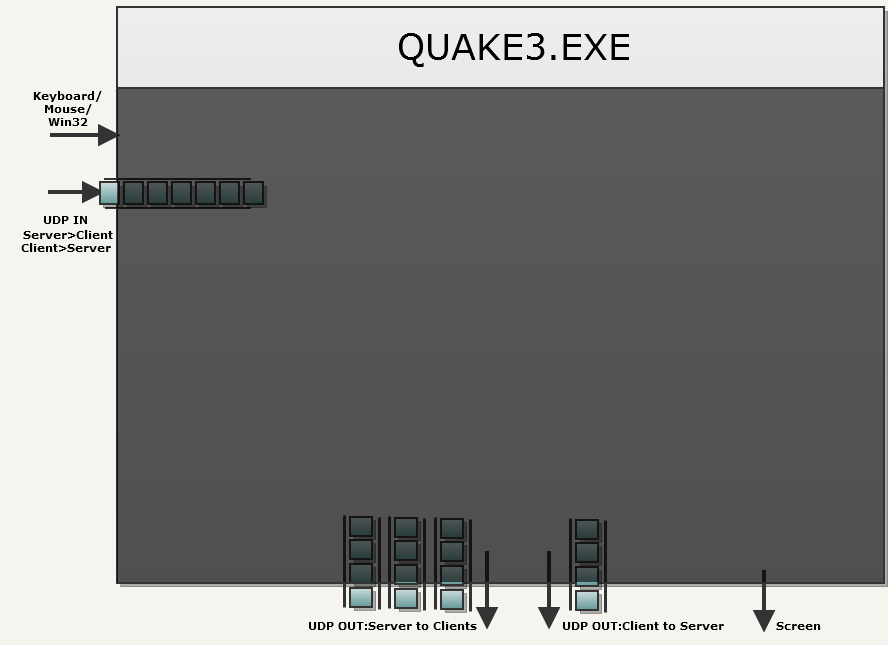
\includegraphics[width=1\textwidth]{images/q3_architecture_blackbox}
			\label{fig:architectureblackbox}
			\caption{Q3 architecture blackbox}
		\end{figure}
	\end{center}

	Dentro del sistema se identifican 6 módulos: lógica de juego (\textit{quake3.exe}), rendering (\textit{renderer.lib}), IA (\textit{bot.lib}), game (\textit{game}), cgame (\textit{cgame}) e interfaz de usuario (\textit{q3\_ui}), representados en la Figura 2 \begin{comment}\ref{fig:architecture}\end{comment} 

		\begin{center}
			\begin{figure}[h]
				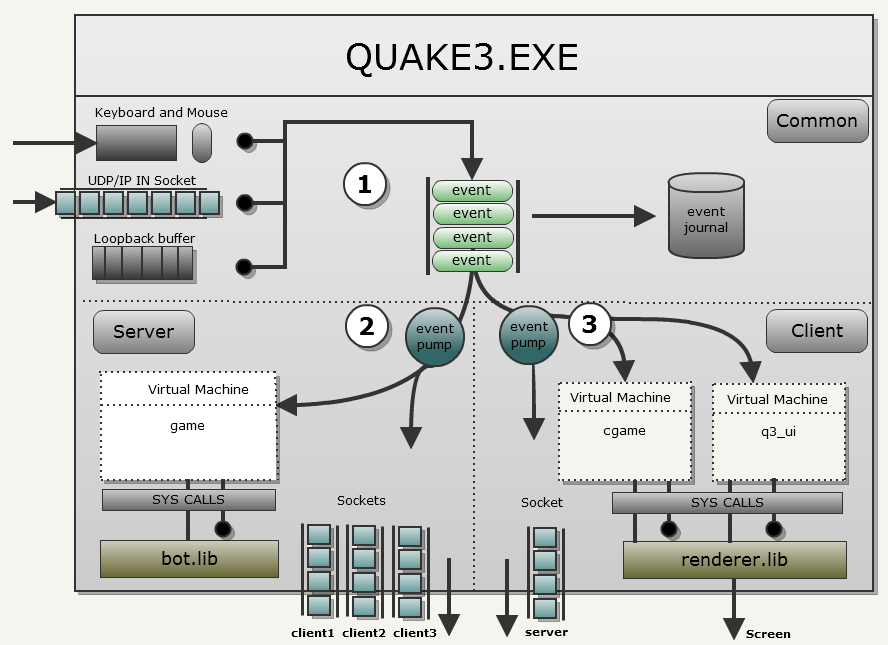
\includegraphics[width=1\textwidth]{images/q3_architecture}
				\label{fig:architecture}
				\caption{Q3 architecture}
			\end{figure}
		\end{center}
	
	En esta arquitectura se destacan dos decisiones de diseño muy importantes:
	
	\subsubsection{Bitácora de inputs para facilitar las pruebas}
	
	Cada uno de los inputs recibidos (Teclado, mensaje win32, ratón, socket UDP) es convertido a \textit{event\_t} y encolado en una cola de eventos (\textit{sysEvent\_t eventQue[256]}). Con esta aproximación se puede mantener una bitácora de estos inputs que, junto con otros factores también almacenados, permiten ser reproducidos en orden para recrear bugs de manera consistente. \cite{johncplan}\\
	
	En la figura X se identifican dentro de la parte \textit{Common} el administrador de inputs, la cola de eventos y el \textit{event journal} mencionado.
	
	\subsubsection{Separación explícita de cliente y servidor}
	
	Durante el desarrollo de \textit{id tech 3} se decidió tomar la decisión de implementar una arquitectura cliente-servidor en la que los roles y subsistemas de cada uno de los dos fueran significativamente distintos. Hasta entonces los clientes y servidores contenían el mismo código pero debían desempeñar roles distintos.\\
	
	En Q3 el servidor es el responsable de mantener el estado de la partida, determinar información de la partida necesitan los clientes y propagarla por la red. Se puede observar en la imagen que \textit{bot.lib} está contenido únicamente dentro de la parte servidora, ya que es también la encargada de proveer la lógica e inputs de los jugadores controlados por la IA.\\
	
	El cliente es responsable de predecir dónde están los objetos en cada instante, incluyendo los elementos afectados por la red utilizando una técnica llamada \textit{lag compensation}, y de renderizar la vista para el usuario \,---\, De nuevo, en la figura X se puede observar como\textit{ renderer.lib} está contenido en la parte cliente. \cite{architecture}\\
    
    \subsubsection{Arquitectura de Red basada en Snapshots}
    
    http://fabiensanglard.net/quake3/network.php
    
    \subsubsection{Quake Virtual Machines}
    
    http://fabiensanglard.net/quake3/qvm.php
	
	\subsubsection{Eventos desde el punto de vista del código}
	
	Para ilustrar la producción/consumición de eventos se puede estudiar el bucle principal (\textit{main}) del código de Q3. Se muestra un ejemplo resumido (Código omitido y desenroscado):
	
	\begin{lstlisting}[style=C, numbers=none]
int WinMain(HINSTANCE hInstance, HINSTANCE hPrevInstance, LPSTR lpCmdLine, int nCmdShow)
{
  Com_Init
	
  NET_Init
	
  while( 1 )
  {
     // Codigo de Common 
    IN_Frame()  // Inyecta los inputs de Win32 joystick y raton en la cola unificada de eventos como event_t.
    {
      IN_JoyMove
      IN_ActivateMouse
      IN_MouseMove
    }
    
    Com_Frame
    {
      // Codigo de Common 
      Com_EventLoop // Envia mensajes win32, paquetes UDP del socket y comandos de la consola a la cola
      (sysEvent_t eventQue[256])
      Cbuf_Execute
      
      // Codigo de Servidor (SV)
      SV_Frame
      {
        SV_BotFrame // Llamada a bot.lib para avanzar su logica
        VM_Call( gvm, GAME_RUN_FRAME, svs.time ) // Llamada a la Game Virtual Machine para procesar la logica de juego
        SV_CheckTimeouts
        SV_SendClientMessages  // Enviar el snapshot o delta snapshot (diferencia entre el snapshot anterior y el actual) a los clientes conectados
      } 
      
      // Codigo de Common aqui
      Com_EventLoop
      Cbuf_Execute
      
      // Codigo de cliente (CL)
      CL_Frame
      {
        CL_SendCmd // Eenviar los comandos al servidor usando la cola de eventos.
        
        SCR_UpdateScreen
        VM_Call( cgvm, CG_DRAW_ACTIVE_FRAME); // Enviar mensajes a la Client Virtual Machine (encargada de hacer las predicciones).
        or
        VM_Call( uivm, UI_DRAW_CONNECT_SCREEN); // Envia un mensaje a la UI Virtual Machine si esta el menu abierto
        
        S_Update // Actualizar los buffers de sonido
      }
    }
  }
}
	\end{lstlisting}

    En este código se puede observar la potencia del patrón basado en máquinas virtuales, que permite obviar las llamadas de renderizado en el bucle principal del juego. Lo único que necesita hacer este bucle es enviar un mensaje (evento) a la máquina virtual del cliente (\textit{CG\_DRAW\_ACTIVE\_FRAME}) indicándole que es necesario realizar un refresco (cargar el siguiente fotograma).\\
    
    Esta máquina virtual realiza los trabajos de culling y predicción antes de llamar a las librerías de OpenGL usando una llamada del sistema Q3 (\textit{CG\_R\_RENDERSCENE}). Cuando Quake.exe recibe esta llamada es cuándo realmente se llama a la función de renderizado de la escena (\textit{RE\_RenderScene}).\cite{unrolled_loop_source}\cite{unrolled_loop}\\   
    
    En la figura X se puede visualizar esta explicación. En lugar de tener todas las llamadas acopladas y dependientes del mismo ciclo de vida, se aprovecha la arquitectura de mensajes para que cada componente realice su trabajo cuando esté listo para procesarlo. Además, esto implica que Quake3.exe no tiene necesidad de saber qué trabajos va a realizar la \textit{Client Virtual Machine} antes de lanzar el mensaje para hacer el render de la escena.\\
    
    

    
	
	
	
	\newpage
	\section{Diseño de Software}
	design patterns and anti-patterns\\
	
	\section{Calidad del Software}
    El software se distribuyó en una única release, ofreciendo el código fuente del motor y unas breves líneas de cómo compilar para Windows, Linux y Mac. No se proporciona más documentación que este breve README, aunque la gente que ha trabajado con este código liberado dice no haber tenido problema para familiarizarse con el código usando los comentarios y la claridad del estilo utilizado, con ficheros y clases bien diferenciadas.\\
    
    No se acompaña el código, tampoco, con ningún tipo de test, por lo que cualquier modificación propia podría introducir cambios y regresiones en las features ya implementadas sin ningún tipo de manera de comprobarlo de manera automática. La filosofía en \textit{id software} era basada en que el testing era una tarea del programador sobre su propio código, además de mediante playtesting diario para comprobar la integración. Es difícil automatizar las tareas de testing para un videojuego online, actualmente se sigue empleando el testing via playtesting entre jugadores reales, pero sí se echan en falta \textit{unit tests} sobre módulos en los que podría encajar hacerlos.\\
    
    Respecto al performance en Q3 se incluyen varias herramientas in-game para medir todo tipo de parámetros relacionados. Podemos distinguir entre dos grandes grupos, las mediciones sobre el performance gráfico (Como los fotogramas por segundo y \textit{frame time}) y las mediciones sobre la red, accesibles mediante la variable \textit{CG\_LAGOMETER}. Con el Lag-o-Meter podemos obtener gráficas sobre el estado de la conexión entre el cliente y el servidor, de esta manera podrían observarse cuellos de botella o problemas en los protocolos de red implementados.
	
	\section{Estado de la accesibilidad en el proyecto}
    Al ser un juego de acción rápida contra oponentes por Internet no existen ningún tipo de consideración para la accesibilidad de ningún tipo. Aún así, existen algunas features que se podrían haber incluído para mejorar la accesibilidad del software como: Paletas de colores para daltónicos, ajustes de brillo y contraste extremos para gente con muy mala vista e indicadores visuales y subtítulos para sordos.
	
	\section{Conclusiones}
	TODO\\
    
	
	
	
	\begin{appendices}
	\end{appendices}
	
	\begin{thebibliography}{9}
		
		\bibitem{example}Google \emph{Ejemplo Bibliografía}. URL: \url{http://www.google.com}\\
		\bibitem{quake3}Quake III Arena \emph{Quake Wikia}. URL: \url{http://quake.wikia.com/wiki/Quake_III_Arena}\\
		\bibitem{idtech3} id tech 3 \emph{Giant Bomb}. URL: \url{https://www.giantbomb.com/id-tech-3/3015-1918/}\\
		\bibitem{sourcecode} Quake III Arena Source Code \emph{Github}. URL: \url{https://github.com/id-Software/Quake-III-Arena}\\
		\bibitem{ioquake3} ioquake3 \emph{ioquake3}. URL: \url{https://ioquake3.org/}
        \bibitem{johncplan} John Carmack's 14 Oct 1998 .plan (Archived from original). \emph{John Carmack}. URL: \url{https://raw.githubusercontent.com/ESWAT/john-carmack-plan-archive/master/by_day/johnc_plan_19981014.txt}
		\bibitem{architecture} Quake 3 Source Code Review. \emph{Fabien Sanglard}. URL: \url{http://fabiensanglard.net/quake3/index.php}
		\bibitem{unrolled_loop_source} Quake 3 Main. \emph{id software}. URL: \url{https://raw.githubusercontent.com/id-Software/Quake-III-Arena/dbe4ddb10315479fc00086f08e25d968b4b43c49/code/win32/win_main.c}
        \bibitem{unrolled_loop} Quake 3 Loop Unrolled. \emph{Fabien Sanglard}. URL: \url{http://fabiensanglard.net/quake3/q3_loop_unrolled.txt}
		
	\end{thebibliography}


	
	
\end{document}
